\section{Model Checking Co-simulation Using Timed Automata}
\label{sec:ma&uppaal}
This section performs a formal analysis of the SysML architectures of water tank shown in Fig.\ref{trs-seq}. First off, we model FMUs which are the components of the SysML architectures and the master algorithm which is the director of FMUs using timed automata in UPPAAL. Next, the verification and analysis checks whether the model is accurate and satisfies certain desired properties. 

\subsection{Modelling FMU component in UPPAAL}
UPPAAL \cite{BehrmannDLHPYH06} is a toolset for verification of real-time systems represented by (a network of) timed automata which is extended with integer variables, structured data types, and channel synchronization. The execution of FMU component and co-simulation is time-related, therefore it is convenient to model the FMU with timed automata in UPPAAL. In this subsection, we abstract the execution of FMU, and encode it with the states and transitions in timed automata. Besides, we also model the master algorithm as a timed automata to coordinate the execution between several FMU components. The timed automata template for FMU components and master algorithm are shown in Fig.\ref{tk-arch1}. Here, we choose rollback algorithm as the master algorithm to coordinate the FMU components. The other two master algorithms can be analyzed with the similar way.

\begin{figure}[htbp]
\centering{
		\subfigure[Timed automata template for FMU controller]{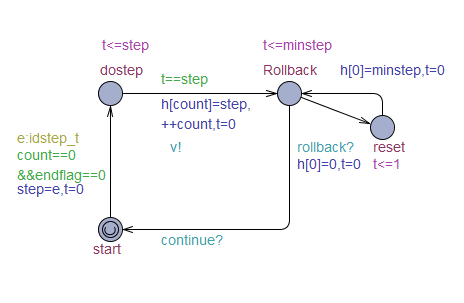
\includegraphics[width=1.6in,height=1.2in]{fig/2signal_controller.png}
			\label{tk_controller}}
		\hfil
		\subfigure[Timed automata for FMU valve]{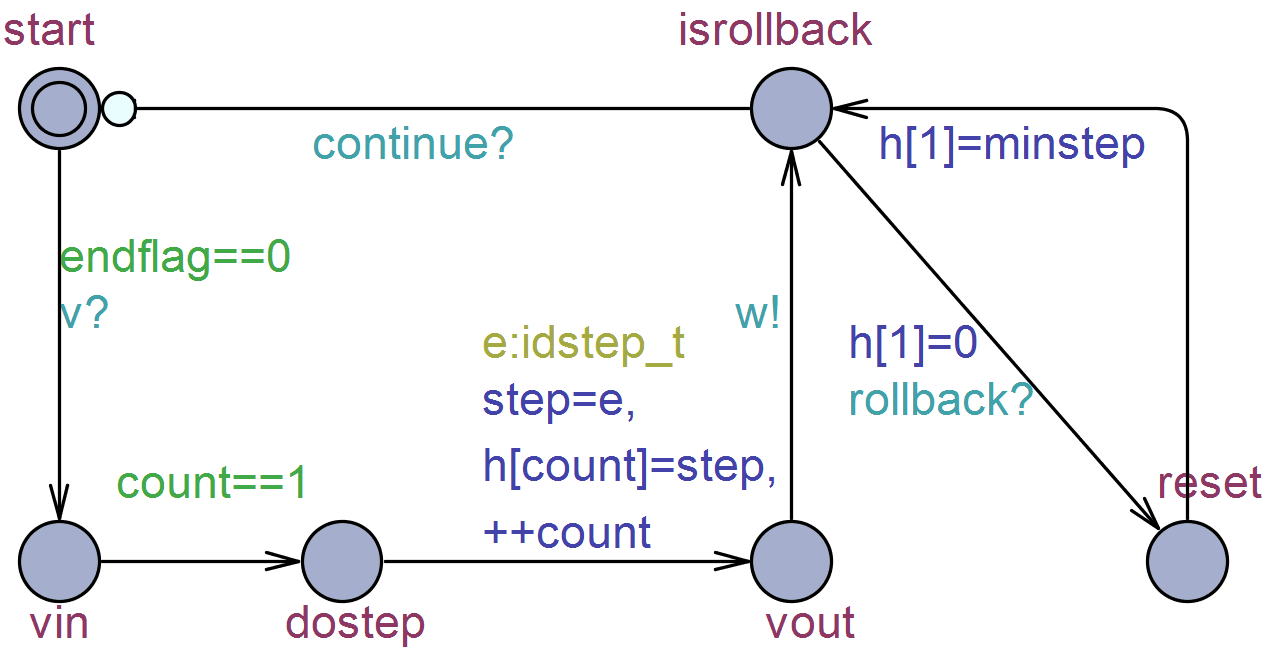
\includegraphics[width=1.6in,height=1.2in]{fig/2signal_v.png}
			\label{tk_v}}
			
	    \subfigure[Timed automata for FMU tank1]{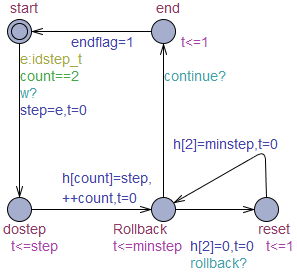
\includegraphics[width=1.5in,height=1.2in]{fig/2signal_wt1.png}
			\label{tk_wt1}}
		\hfil
		 \subfigure[Timed automata for master algorithm]{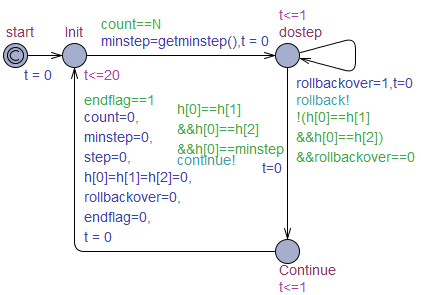
\includegraphics[width=1.7in,height=1.2in]{fig/2signal_master.png}
			\label{tk_ma}}		
	\caption{Timed automata templates for connection case 1.}
	\label{tk-arch1}
	}
\end{figure}

\begin{figure}[htbp]
\centering{
		\subfigure[Execution trace]{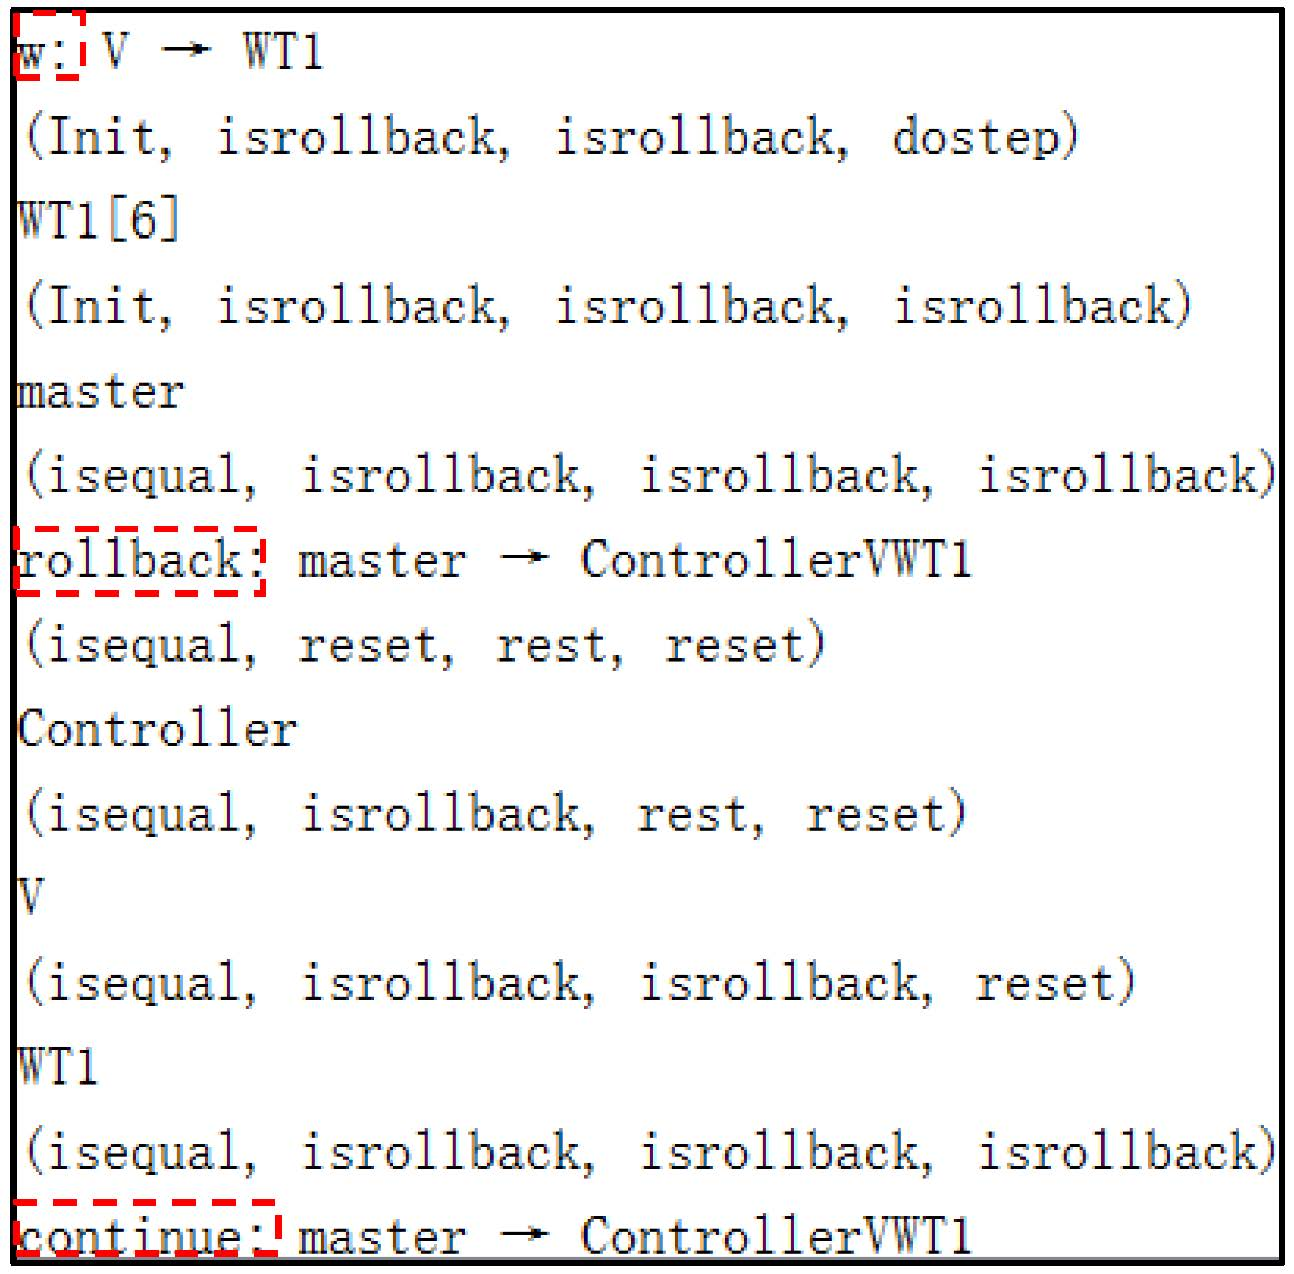
\includegraphics[width=1.6in,height=1.8in]{fig/trs.jpg}
			\label{trs}}
		\hfil
		\subfigure[Execution sequence diagram]{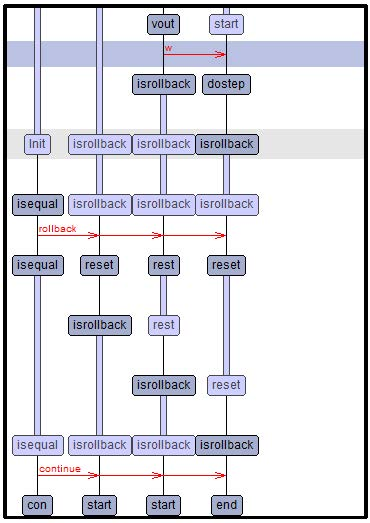
\includegraphics[width=1.6in,height=1.8in]{fig/seq.jpg}
			\label{seq}}
	\caption{The execution fragment of the co-simulation.}
	\label{trs-seq}
	}
\end{figure}

Figure~\ref{tk_controller}, \ref{tk_v}, \ref{tk_wt1} are the templates for controller, valve and tank1 respectively, they model FMU components which supports rollback function. These FMU components contain four main states, e.g., $start$, $dostep$, $isrollback$ and $reset$. Figure~ \ref{tk_controller} shows the template for controller which supports a random step size. It synchronizes with valve by signal $v$ and jump to $isrollback$ state, and then waits for a signal from the timed automata for the master algorithm. Until the controller receives the $continue$ signal, it does data exchange, and return to $start$ state. Otherwise it receives $rollback$ signal, once it obtains the minimize step size of all FMU components, it travels to $isrollback$ state. The states and transitions of valve and tank1 template are similar with the template of controller. Figure~\ref{tk_ma} shows the template for the master algorithm. Firstly, the master algorithm initialize the parameters, and then it get minimize step size of FMU components until all FMU components visit $dostep$. Next, the master algorithm decides which signal should be sent according to the guard. If the step sizes of all FMU components are equal, the master algorithm will send $continue$ signal, otherwise, send $rollback$ signal.

Figure~\ref{trs-seq} is the execution fragment of the co-simulation, we can find that valve send a $w$ signal to perform data exchange with tank1. After that tank1 move to $dostep$ state. The master algorithm send a $rollback$ signal to all templates, which leads to all of them arrive at $reset$ state. Finally, the master algorithm send a $continue$ signal to others. All templates return to $start$ state, and then do next step. The execution process shows that our model performs correctly.

In order to compare the behavior of three connection cases of water tank presented in Section 4.2, we also model the other two connection cases in UPPAAL. We add a channel $s$ to the templates for controller and tank1, which is the model of connection case 2 as shown in Fig.\ref{tk-arch2}. We add a template (tank2) and channel $w2$, which is the model of connection case 3 shown in Fig.\ref{arc3}. In next subsection, we verify some properties of various connection cases to analyse the correctness of the architecture.
\begin{figure}[htbp]
\centering{
		\subfigure[Timed automata for FMU controller]{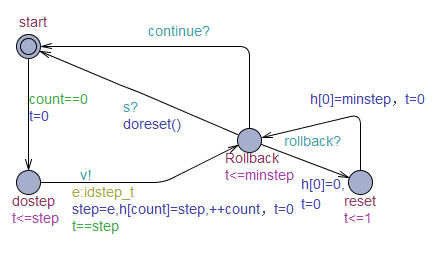
\includegraphics[width=1.8in,height=1.2in]{fig/2signal_cycle_controller.png}
			\label{tk2_controller}}
		\hfil
		\subfigure[Timed automata for FMU tank1]{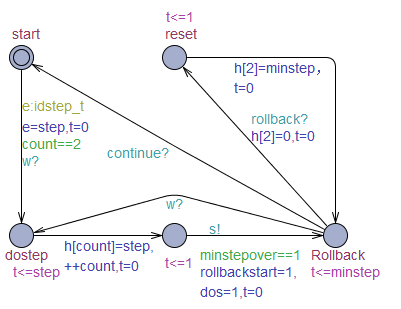
\includegraphics[width=1.5in,height=1.2in]{fig/2signal_cycle_wt1.png}
			\label{tk2_v}}		
	\caption{Timed automata for connection case 2.}
	\label{tk-arch2}
	}
\end{figure}
\begin{figure}[htbp]
	\centering	{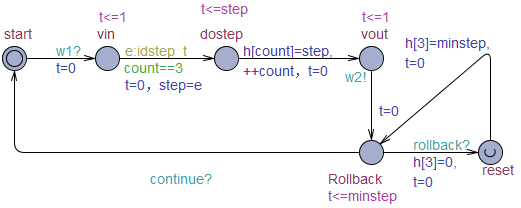
\includegraphics[width=3.0in,height=0.8in]{fig/4signal_wt2.png}}
	\caption{Timed automata for connection case 3.}\label{arc3}
\end{figure}
\subsection{Verification and Analysis}
UPPAAL uses a simplified version of TCTL \cite{BouchenebGR09} to express the requirement specification. We verify the following TCTL properties of each connection case:
\begin{itemize}
\item
$E\langle\rangle~WT1.isrollback$ and $E\langle\rangle~master.con$ are reachability properties checking whether FMU tank1 can reach $isrollback$ state and whether the master algorithm can reach $con$ state respectively.
\item
$master.start \rightarrow master.con$ are liveness property. If the master algorithm arrive at $start$ state, it eventually reaches $con$ state.
\item 
$A[]~not~deadlock$ is safety property checking whether the model will be deadlock.
\end{itemize}

The verification results are shown in Table\ref{rs}. We can find that all properties of connection case 1 and 3 are satisfied. It proves that our master algorithm is correct and the composition of FMU components is determinate. However, the liveness and reachability properties of connection case 2 are not satisfied. We find that there is a algebraic loop which may be introduced with the I/O dependency in this connection case. The experiments show that our approach is feasible and useful for model checking the FMI co-simulation. The approach facilitates the verification of the CPSs architecture models.
\begin{table}
\caption{Experimental results}
\centering
\begin{tabular}{c c c} 
        \hline  
        Connection case & Property & Result\\
        \hline
        \multirow{2}{2.0cm}{Case 1}  
                & $E\langle\rangle~WT1.isrollback$ & True\\ 
                & $E\langle\rangle~master.con$ & True\\ 
                & $master.start\rightarrow master.con$ & True\\ 
                & $A[]~not~deadlock$ & True\\   
        \hline 
        \multirow{2}{2.0cm}{Case 2}  
                & $E\langle\rangle~WT1.isrollback$ & True\\ 
                & $E\langle\rangle~master.con$ & False\\ 
                & $master.start\rightarrow master.con$ & False\\ 
                & $A[]~not~deadlock$ & True\\   
        \hline 
        \multirow{2}{2.0cm}{Case 3}  
                & $E\langle\rangle~WT1.isrollback$ & True\\ 
                & $E\langle\rangle~master.con$ & True\\ 
                & $master.start \rightarrow master.con$ & True\\ 
                & $A[]~not~deadlock$ & True\\   
        \hline 
\end{tabular} 
\label{rs}
\end{table}




